% Options for packages loaded elsewhere
\PassOptionsToPackage{unicode}{hyperref}
\PassOptionsToPackage{hyphens}{url}
\PassOptionsToPackage{dvipsnames,svgnames,x11names}{xcolor}
%
\documentclass[
  12pt,
  letterpaper,
  DIV=11,
  numbers=noendperiod,
  oneside]{scrreport}

\usepackage{amsmath,amssymb}
\usepackage{iftex}
\ifPDFTeX
  \usepackage[T1]{fontenc}
  \usepackage[utf8]{inputenc}
  \usepackage{textcomp} % provide euro and other symbols
\else % if luatex or xetex
  \usepackage{unicode-math}
  \defaultfontfeatures{Scale=MatchLowercase}
  \defaultfontfeatures[\rmfamily]{Ligatures=TeX,Scale=1}
\fi
\usepackage{lmodern}
\ifPDFTeX\else  
    % xetex/luatex font selection
  \setmainfont[]{Arial}
\fi
% Use upquote if available, for straight quotes in verbatim environments
\IfFileExists{upquote.sty}{\usepackage{upquote}}{}
\IfFileExists{microtype.sty}{% use microtype if available
  \usepackage[]{microtype}
  \UseMicrotypeSet[protrusion]{basicmath} % disable protrusion for tt fonts
}{}
\makeatletter
\@ifundefined{KOMAClassName}{% if non-KOMA class
  \IfFileExists{parskip.sty}{%
    \usepackage{parskip}
  }{% else
    \setlength{\parindent}{0pt}
    \setlength{\parskip}{6pt plus 2pt minus 1pt}}
}{% if KOMA class
  \KOMAoptions{parskip=half}}
\makeatother
\usepackage{xcolor}
\usepackage[top=30mm,bottom=30mm,left=30mm,right=30mm,heightrounded]{geometry}
\setlength{\emergencystretch}{3em} % prevent overfull lines
\setcounter{secnumdepth}{5}
% Make \paragraph and \subparagraph free-standing
\ifx\paragraph\undefined\else
  \let\oldparagraph\paragraph
  \renewcommand{\paragraph}[1]{\oldparagraph{#1}\mbox{}}
\fi
\ifx\subparagraph\undefined\else
  \let\oldsubparagraph\subparagraph
  \renewcommand{\subparagraph}[1]{\oldsubparagraph{#1}\mbox{}}
\fi


\providecommand{\tightlist}{%
  \setlength{\itemsep}{0pt}\setlength{\parskip}{0pt}}\usepackage{longtable,booktabs,array}
\usepackage{calc} % for calculating minipage widths
% Correct order of tables after \paragraph or \subparagraph
\usepackage{etoolbox}
\makeatletter
\patchcmd\longtable{\par}{\if@noskipsec\mbox{}\fi\par}{}{}
\makeatother
% Allow footnotes in longtable head/foot
\IfFileExists{footnotehyper.sty}{\usepackage{footnotehyper}}{\usepackage{footnote}}
\makesavenoteenv{longtable}
\usepackage{graphicx}
\makeatletter
\def\maxwidth{\ifdim\Gin@nat@width>\linewidth\linewidth\else\Gin@nat@width\fi}
\def\maxheight{\ifdim\Gin@nat@height>\textheight\textheight\else\Gin@nat@height\fi}
\makeatother
% Scale images if necessary, so that they will not overflow the page
% margins by default, and it is still possible to overwrite the defaults
% using explicit options in \includegraphics[width, height, ...]{}
\setkeys{Gin}{width=\maxwidth,height=\maxheight,keepaspectratio}
% Set default figure placement to htbp
\makeatletter
\def\fps@figure{htbp}
\makeatother
% definitions for citeproc citations
\NewDocumentCommand\citeproctext{}{}
\NewDocumentCommand\citeproc{mm}{%
  \begingroup\def\citeproctext{#2}\cite{#1}\endgroup}
\makeatletter
 % allow citations to break across lines
 \let\@cite@ofmt\@firstofone
 % avoid brackets around text for \cite:
 \def\@biblabel#1{}
 \def\@cite#1#2{{#1\if@tempswa , #2\fi}}
\makeatother
\newlength{\cslhangindent}
\setlength{\cslhangindent}{1.5em}
\newlength{\csllabelwidth}
\setlength{\csllabelwidth}{3em}
\newenvironment{CSLReferences}[2] % #1 hanging-indent, #2 entry-spacing
 {\begin{list}{}{%
  \setlength{\itemindent}{0pt}
  \setlength{\leftmargin}{0pt}
  \setlength{\parsep}{0pt}
  % turn on hanging indent if param 1 is 1
  \ifodd #1
   \setlength{\leftmargin}{\cslhangindent}
   \setlength{\itemindent}{-1\cslhangindent}
  \fi
  % set entry spacing
  \setlength{\itemsep}{#2\baselineskip}}}
 {\end{list}}
\usepackage{calc}
\newcommand{\CSLBlock}[1]{\hfill\break\parbox[t]{\linewidth}{\strut\ignorespaces#1\strut}}
\newcommand{\CSLLeftMargin}[1]{\parbox[t]{\csllabelwidth}{\strut#1\strut}}
\newcommand{\CSLRightInline}[1]{\parbox[t]{\linewidth - \csllabelwidth}{\strut#1\strut}}
\newcommand{\CSLIndent}[1]{\hspace{\cslhangindent}#1}

\KOMAoption{captions}{tableheading}
\usepackage[dvipsnames]{xcolor}
\usepackage[T1]{fontenc}
\makeatletter
\@ifpackageloaded{tcolorbox}{}{\usepackage[skins,breakable]{tcolorbox}}
\@ifpackageloaded{fontawesome5}{}{\usepackage{fontawesome5}}
\definecolor{quarto-callout-color}{HTML}{909090}
\definecolor{quarto-callout-note-color}{HTML}{0758E5}
\definecolor{quarto-callout-important-color}{HTML}{CC1914}
\definecolor{quarto-callout-warning-color}{HTML}{EB9113}
\definecolor{quarto-callout-tip-color}{HTML}{00A047}
\definecolor{quarto-callout-caution-color}{HTML}{FC5300}
\definecolor{quarto-callout-color-frame}{HTML}{acacac}
\definecolor{quarto-callout-note-color-frame}{HTML}{4582ec}
\definecolor{quarto-callout-important-color-frame}{HTML}{d9534f}
\definecolor{quarto-callout-warning-color-frame}{HTML}{f0ad4e}
\definecolor{quarto-callout-tip-color-frame}{HTML}{02b875}
\definecolor{quarto-callout-caution-color-frame}{HTML}{fd7e14}
\makeatother
\makeatletter
\@ifpackageloaded{bookmark}{}{\usepackage{bookmark}}
\makeatother
\makeatletter
\@ifpackageloaded{caption}{}{\usepackage{caption}}
\AtBeginDocument{%
\ifdefined\contentsname
  \renewcommand*\contentsname{Tabla de contenidos}
\else
  \newcommand\contentsname{Tabla de contenidos}
\fi
\ifdefined\listfigurename
  \renewcommand*\listfigurename{Listado de Figuras}
\else
  \newcommand\listfigurename{Listado de Figuras}
\fi
\ifdefined\listtablename
  \renewcommand*\listtablename{Listado de Tablas}
\else
  \newcommand\listtablename{Listado de Tablas}
\fi
\ifdefined\figurename
  \renewcommand*\figurename{Figura}
\else
  \newcommand\figurename{Figura}
\fi
\ifdefined\tablename
  \renewcommand*\tablename{Tabla}
\else
  \newcommand\tablename{Tabla}
\fi
}
\@ifpackageloaded{float}{}{\usepackage{float}}
\floatstyle{ruled}
\@ifundefined{c@chapter}{\newfloat{codelisting}{h}{lop}}{\newfloat{codelisting}{h}{lop}[chapter]}
\floatname{codelisting}{Listado}
\newcommand*\listoflistings{\listof{codelisting}{Listado de Listados}}
\makeatother
\makeatletter
\makeatother
\makeatletter
\@ifpackageloaded{caption}{}{\usepackage{caption}}
\@ifpackageloaded{subcaption}{}{\usepackage{subcaption}}
\makeatother
\makeatletter
\@ifpackageloaded{sidenotes}{}{\usepackage{sidenotes}}
\@ifpackageloaded{marginnote}{}{\usepackage{marginnote}}
\makeatother
\ifLuaTeX
\usepackage[bidi=basic]{babel}
\else
\usepackage[bidi=default]{babel}
\fi
\babelprovide[main,import]{spanish}
\ifPDFTeX
\else
\babelfont{rm}[]{Arial}
\fi
% get rid of language-specific shorthands (see #6817):
\let\LanguageShortHands\languageshorthands
\def\languageshorthands#1{}
\ifLuaTeX
  \usepackage{selnolig}  % disable illegal ligatures
\fi
\usepackage{bookmark}

\IfFileExists{xurl.sty}{\usepackage{xurl}}{} % add URL line breaks if available
\urlstyle{same} % disable monospaced font for URLs
\hypersetup{
  pdflang={es},
  colorlinks=true,
  linkcolor={RoyalBlue},
  filecolor={Blue},
  citecolor={Goldenrod},
  urlcolor={RoyalBlue},
  pdfcreator={LaTeX via pandoc}}

\author{}
\date{}

\begin{document}

\renewcommand*\contentsname{Tabla de contenidos}
{
\hypersetup{linkcolor=Black}
\setcounter{tocdepth}{2}
\tableofcontents
}
\listoffigures
\listoftables
\bookmarksetup{startatroot}

\chapter*{Preface}\label{preface}
\addcontentsline{toc}{chapter}{Preface}

\markboth{Preface}{Preface}

Este es un libro o tesis creado con \textbf{Quarto}

Para aprender más sobre Quarto books visita:
\url{https://quarto.org/docs/books}.

\bookmarksetup{startatroot}

\chapter*{Agradecimientos}\label{agradecimientos}
\addcontentsline{toc}{chapter}{Agradecimientos}

\markboth{Agradecimientos}{Agradecimientos}

\begin{quote}
Aliquam erat volutpat. Nullam vel augue fringilla, tempor lacus vitae,
viverra magna. Aenean dictum volutpat metus vehicula imperdiet. Donec
vitae placerat purus. Suspendisse potenti. Suspendisse tincidunt at nibh
sit amet pulvinar. Suspendisse non eros dignissim, lacinia justo in,
vulputate magna. Nullam sed libero convallis, consequat nisl sed,
facilisis odio. Nam tincidunt ut arcu id convallis. Donec eget auctor
sem. Mauris in porttitor sem. Mauris id condimentum massa. Aenean
lacinia, mauris sed bibendum laoreet, velit quam fringilla mauris, eu
hendrerit quam libero nec urna. Pellentesque aliquet erat quis ante
commodo lacinia. In quis elit arcu.
\end{quote}

\begin{titlepage}
    \begin{center}
        \vspace*{0.5cm}
        
        \Large
        \textbf{UNIVERSIDAD NACIONAL AUTÓNOMA DE MÉXICO}
        
        
\includegraphics[width=0.2\textwidth]{cover.png}
        
        \vspace{0.5cm}
        
        \vspace{0.5cm}
        \Large
        Maestría y Doctorado en Ciencias Bioquímicas
        
        \vspace{1.5cm}
        
        \LARGE
        \textbf{(TÍTULO DEL TRABAJO)}
        
        \vspace{1.5cm}
        
        \textbf{TESIS}
        
        \vspace{0.5cm}
        
        \Large
        QUE PARA OPTAR POR EL GRADO DE:
        
        \vspace{0.5cm}
        
        \textbf{Doctor en Ciencias}
        
        \vspace{0.5cm}
        
        \Large
        PRESENTA:
        
        \vspace{0.5cm}
        
        \textbf{(NOMBRE DEL ALUMNO)}
        
        \vfill
        
        \Large
        TUTOR PRINCIPAL \\
        Entidad de adscripción
        
        \vspace{0.5cm}
        
        \Large
        MIEMBROS DEL COMITÉ TUTOR \\
        Entidad de adscripción
        
        \vspace{0.7cm}
        
        \Large
        Ciudad de México, mes, 201--
        
    \end{center}
\end{titlepage}

\bookmarksetup{startatroot}

\chapter{Summary}\label{summary}

In summary, this book has no content whatsoever.

\bookmarksetup{startatroot}

\chapter{Introducción}\label{sec-Introduccion}

Aquí hay un footnote \footnote{Así aparece tu footnote}

\begin{tcolorbox}[enhanced jigsaw, bottomrule=.15mm, toprule=.15mm, opacityback=0, rightrule=.15mm, colback=white, breakable, left=2mm, arc=.35mm, colframe=quarto-callout-tip-color-frame, leftrule=.75mm]

\vspace{-3mm}\textbf{Aquí va tip:}\vspace{3mm}

\end{tcolorbox}

\section{Una cita}\label{una-cita}

Aquí va una cita con el \texttt{.csl} de plosOne que viene en este
template. Knuth (\citeproc{ref-knuth84}{1984}). Puedes cambiar o buscar
en internet el .csl y cambiarlo en el Archivo que con extensión
\texttt{.YML}

\section{Experimental}\label{experimental}

Aliquam erat volutpat. Nullam vel augue fringilla, tempor lacus vitae,
viverra magna. Aenean dictum volutpat metus vehicula imperdiet. Donec
vitae placerat purus. Suspendisse potenti. Suspendisse tincidunt at nibh
sit amet pulvinar. Suspendisse non eros dignissim, lacinia justo in,
vulputate magna. Nullam sed libero convallis, consequat nisl sed,
facilisis odio. Nam tincidunt ut arcu id convallis. Donec eget auctor
sem. Mauris in porttitor sem. Mauris id condimentum massa. Aenean
lacinia, mauris sed bibendum laoreet, velit quam fringilla mauris, eu
hendrerit quam libero nec urna. Pellentesque aliquet erat quis ante
commodo lacinia. In quis elit arcu Tabla~\ref{tbl-example}.
Tabla~\ref{tbl-los_promedios} Notice that the caption is positioned at
the top of the table.

\begin{longtable}[]{@{}ll@{}}
\caption{An example table}\label{tbl-example}\tabularnewline
\toprule\noalign{}
Header one & Header two \\
\midrule\noalign{}
\endfirsthead
\toprule\noalign{}
Header one & Header two \\
\midrule\noalign{}
\endhead
\bottomrule\noalign{}
\endlastfoot
Entry one & Entry two \\
Entry three & Entry four \\
Entry five & Entry six \\
Entry seven & Entry eight \\
\end{longtable}

\begin{longtable}[]{@{}llll@{}}
\caption{Esta es una tabla de
promedios}\label{tbl-los_promedios}\tabularnewline
\toprule\noalign{}
Juego & Compañia & Clasificacion & Precio (MXN) \\
\midrule\noalign{}
\endfirsthead
\toprule\noalign{}
Juego & Compañia & Clasificacion & Precio (MXN) \\
\midrule\noalign{}
\endhead
\bottomrule\noalign{}
\endlastfoot
Animal Crossing & Nintendo & E & 1600 \\
Persona 5 & Atlus & T & 1500 \\
Final Fantasy VII & Square Enix & T & 1500 \\
Fortnite & Epic Games & M & 0 \\
\end{longtable}

You may add footnotes to ables as illustrated (Tabla~\ref{tbl-notes}).

\begin{longtable}[]{@{}ll@{}}
\caption{An example table with notes}\label{tbl-notes}\tabularnewline
\toprule\noalign{}
Header one & Header two \\
\midrule\noalign{}
\endfirsthead
\toprule\noalign{}
Header one & Header two \\
\midrule\noalign{}
\endhead
\bottomrule\noalign{}
\endlastfoot
Entry one\footnote{This is a footnote} & Entry two \\
Entry three\footnote{This is a second note} & Entry four \\
Entry five & Entry six \\
Entry seven & Entry eight \\
\end{longtable}

\begin{figure}

\centering{

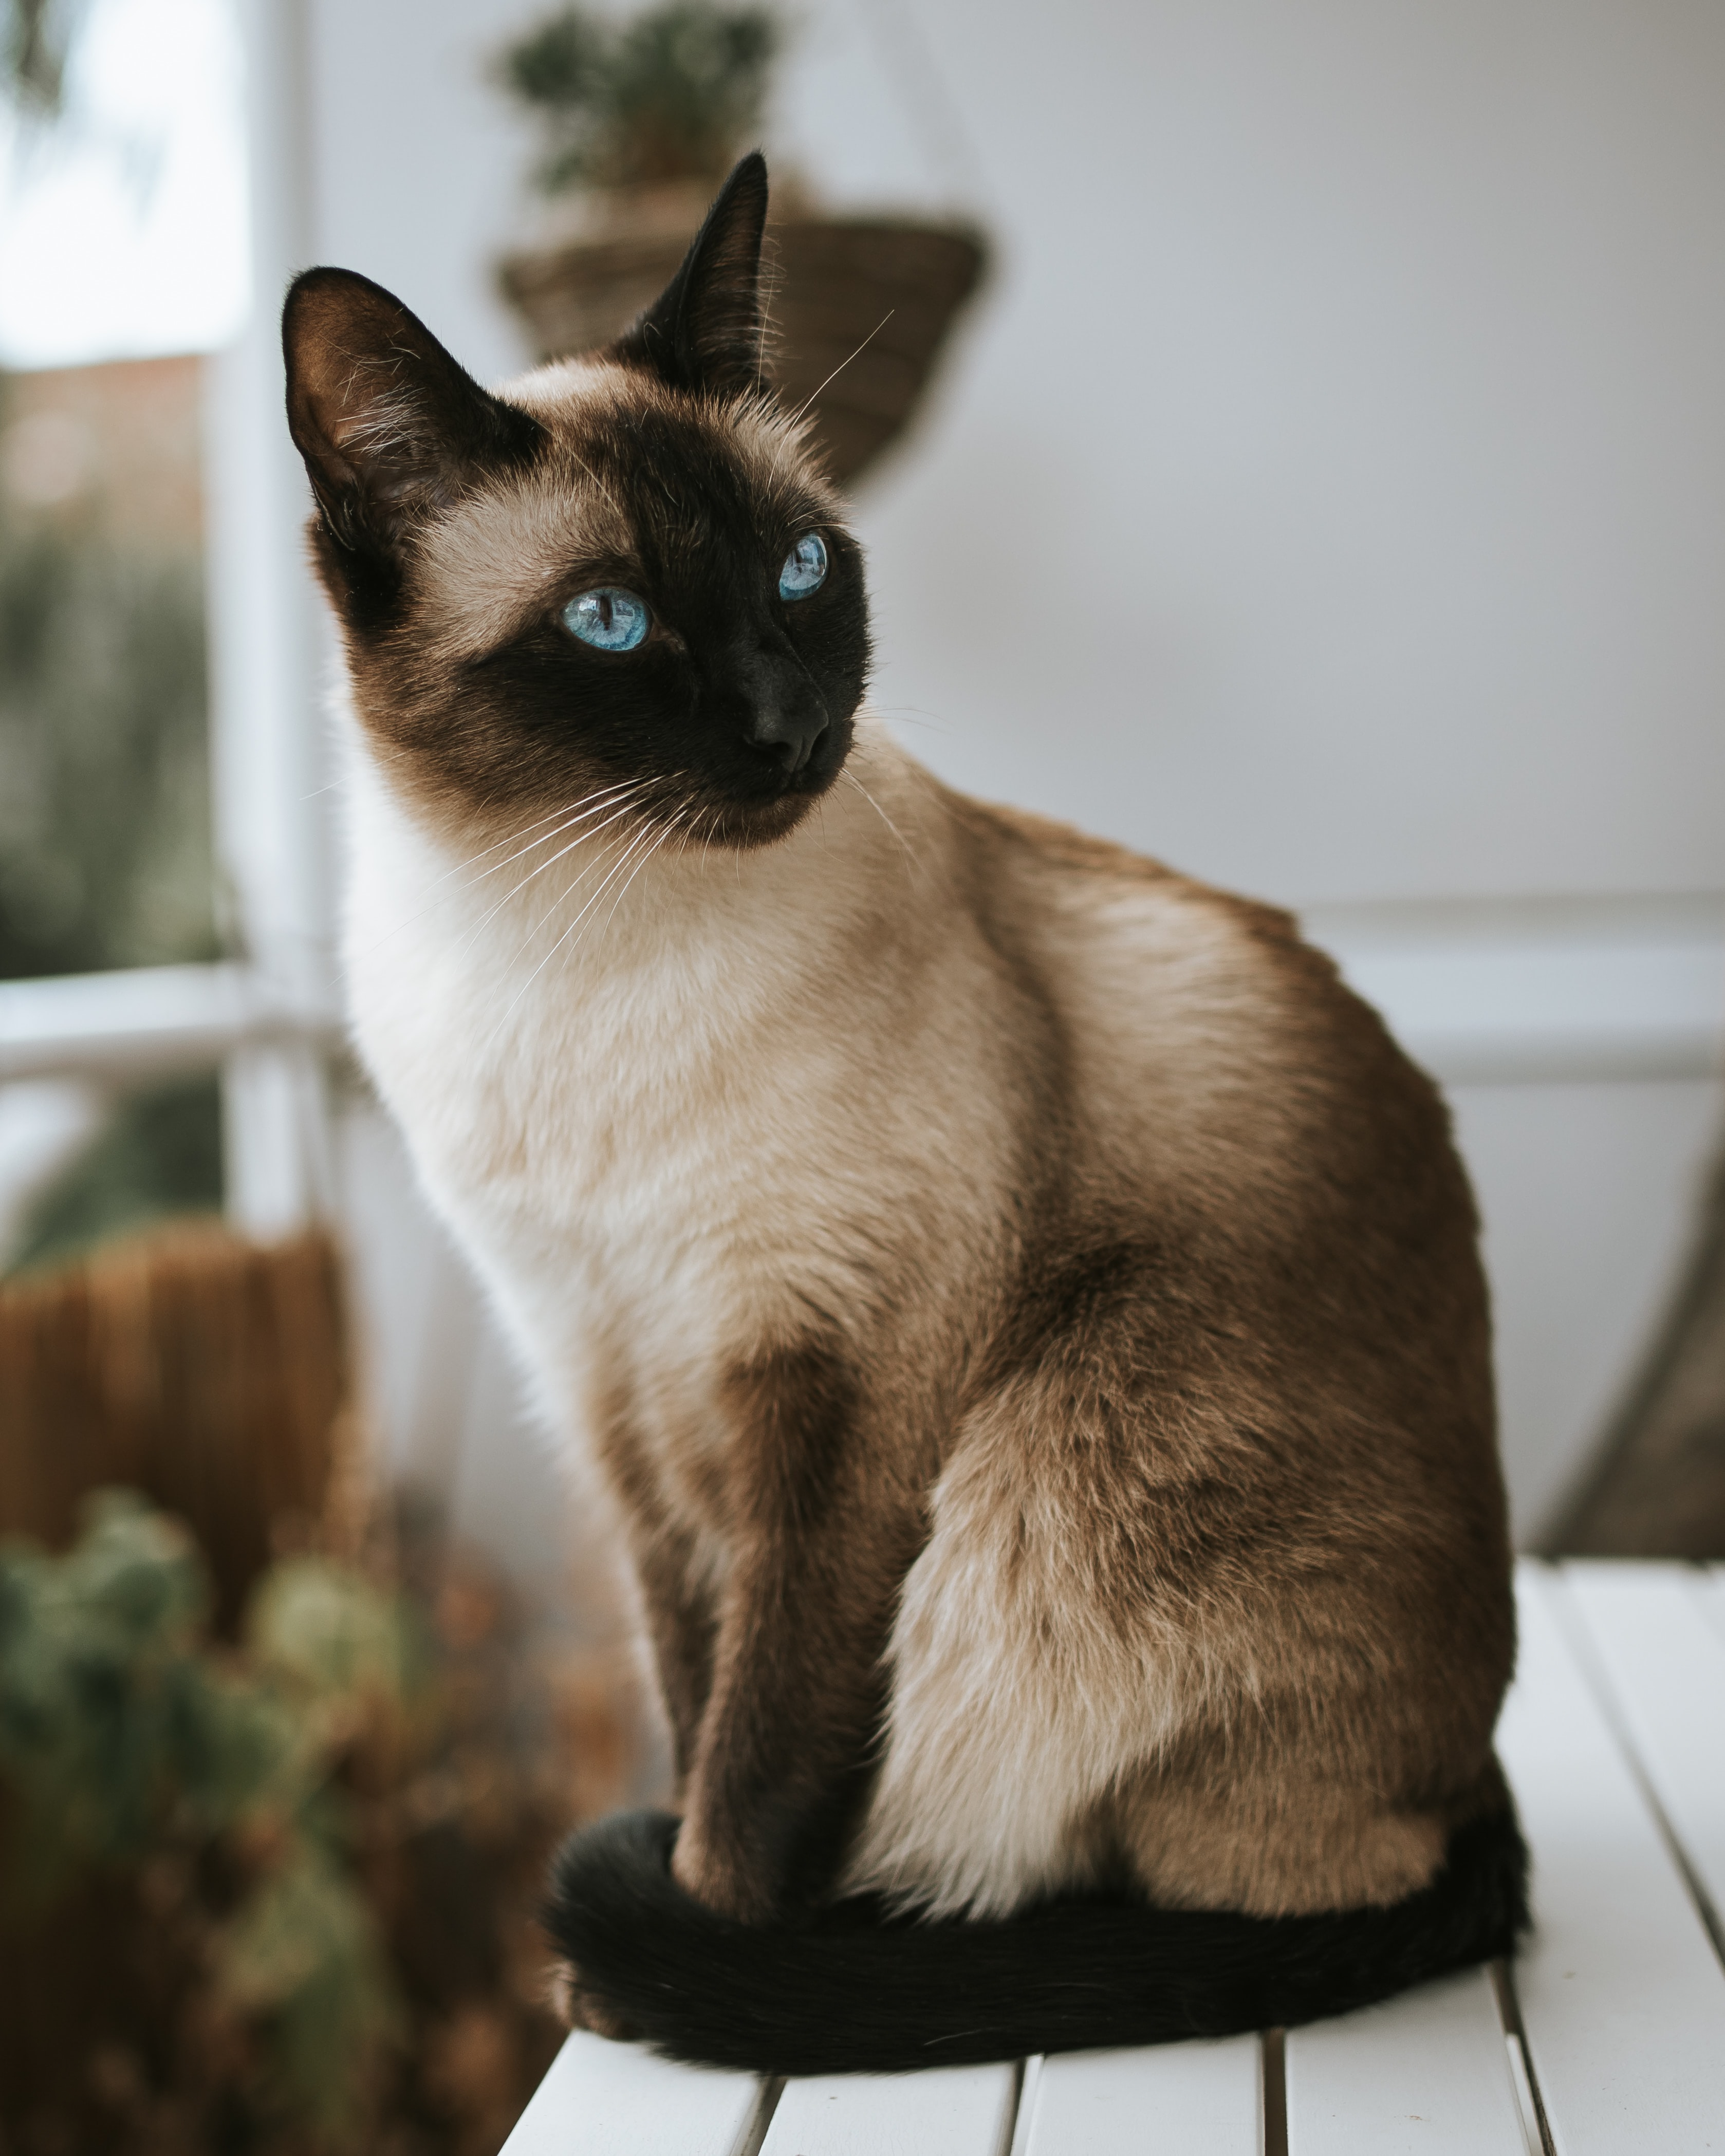
\includegraphics{imagenes/gato_siames.jpg}

}

\caption{\label{fig-gatosiames}Un ejemplo de esquema}

\end{figure}%

La figura Figura~\ref{fig-gatosiames} de un gato siamés.Duis in neque
pellentesque tortor pellentesque tristique. Duis rutrum lectus odio, nec
posuere leo dignissim sit amet. Ut euismod tincidunt mauris. Nullam
pellentesque luctus rutrum. Aenean ut convallis nisl, a efficitur nibh.
Ut urna nulla, lobortis id aliquam at, imperdiet nec sapien. Aenean nec
sem lorem. Maecenas id tempor sem, eu iaculis dolor. Maecenas
pellentesque magna sed nunc iaculis ultricies. In hac habitasse platea
dictumst. Proin tincidunt fringilla molestie. Maecenas euismod fermentum
dolor, non vestibulum justo accumsan eu. Donec venenatis consectetur
lacus, ac auctor mauris porttitor at. Vestibulum bibendum nisl vel
elementum malesuada. Sed a placerat lacus, convallis maximus orci.

\begin{figure}

\begin{minipage}{0.50\linewidth}

\centering{

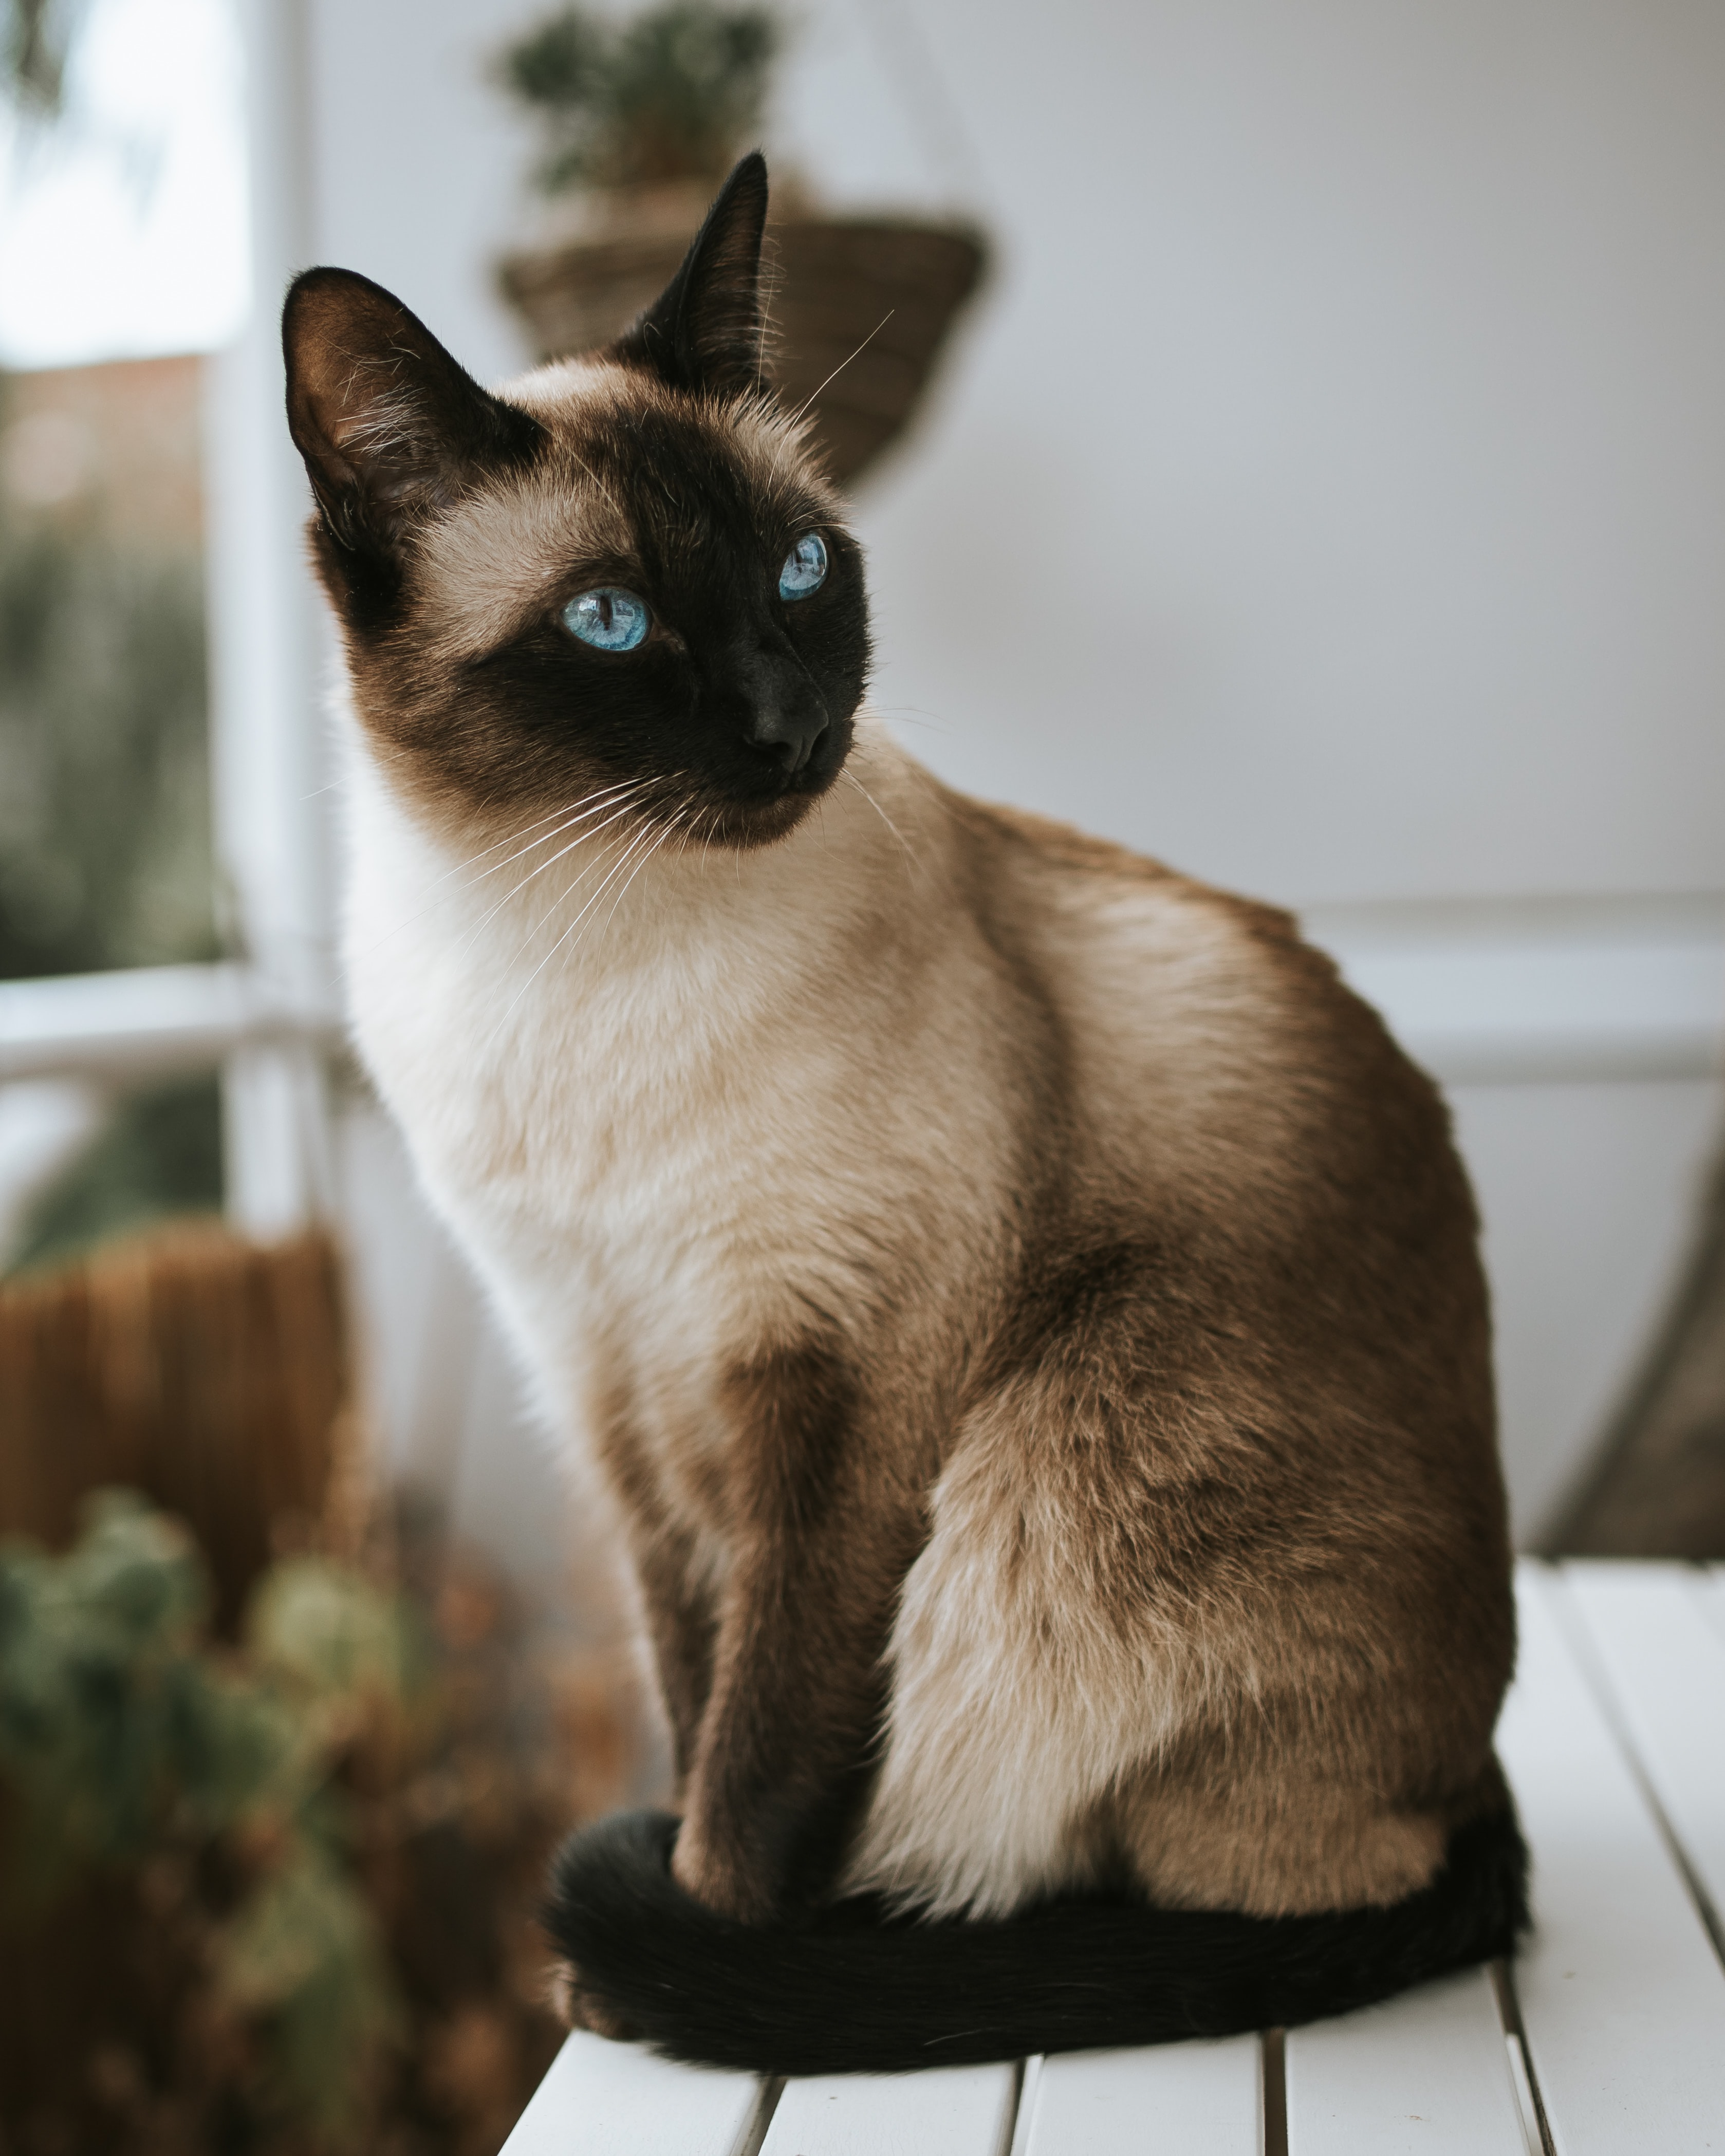
\includegraphics{imagenes/gato_siames.jpg}

}

\subcaption{\label{fig-gato1}gato1}

\end{minipage}%
%
\begin{minipage}{0.50\linewidth}

\centering{

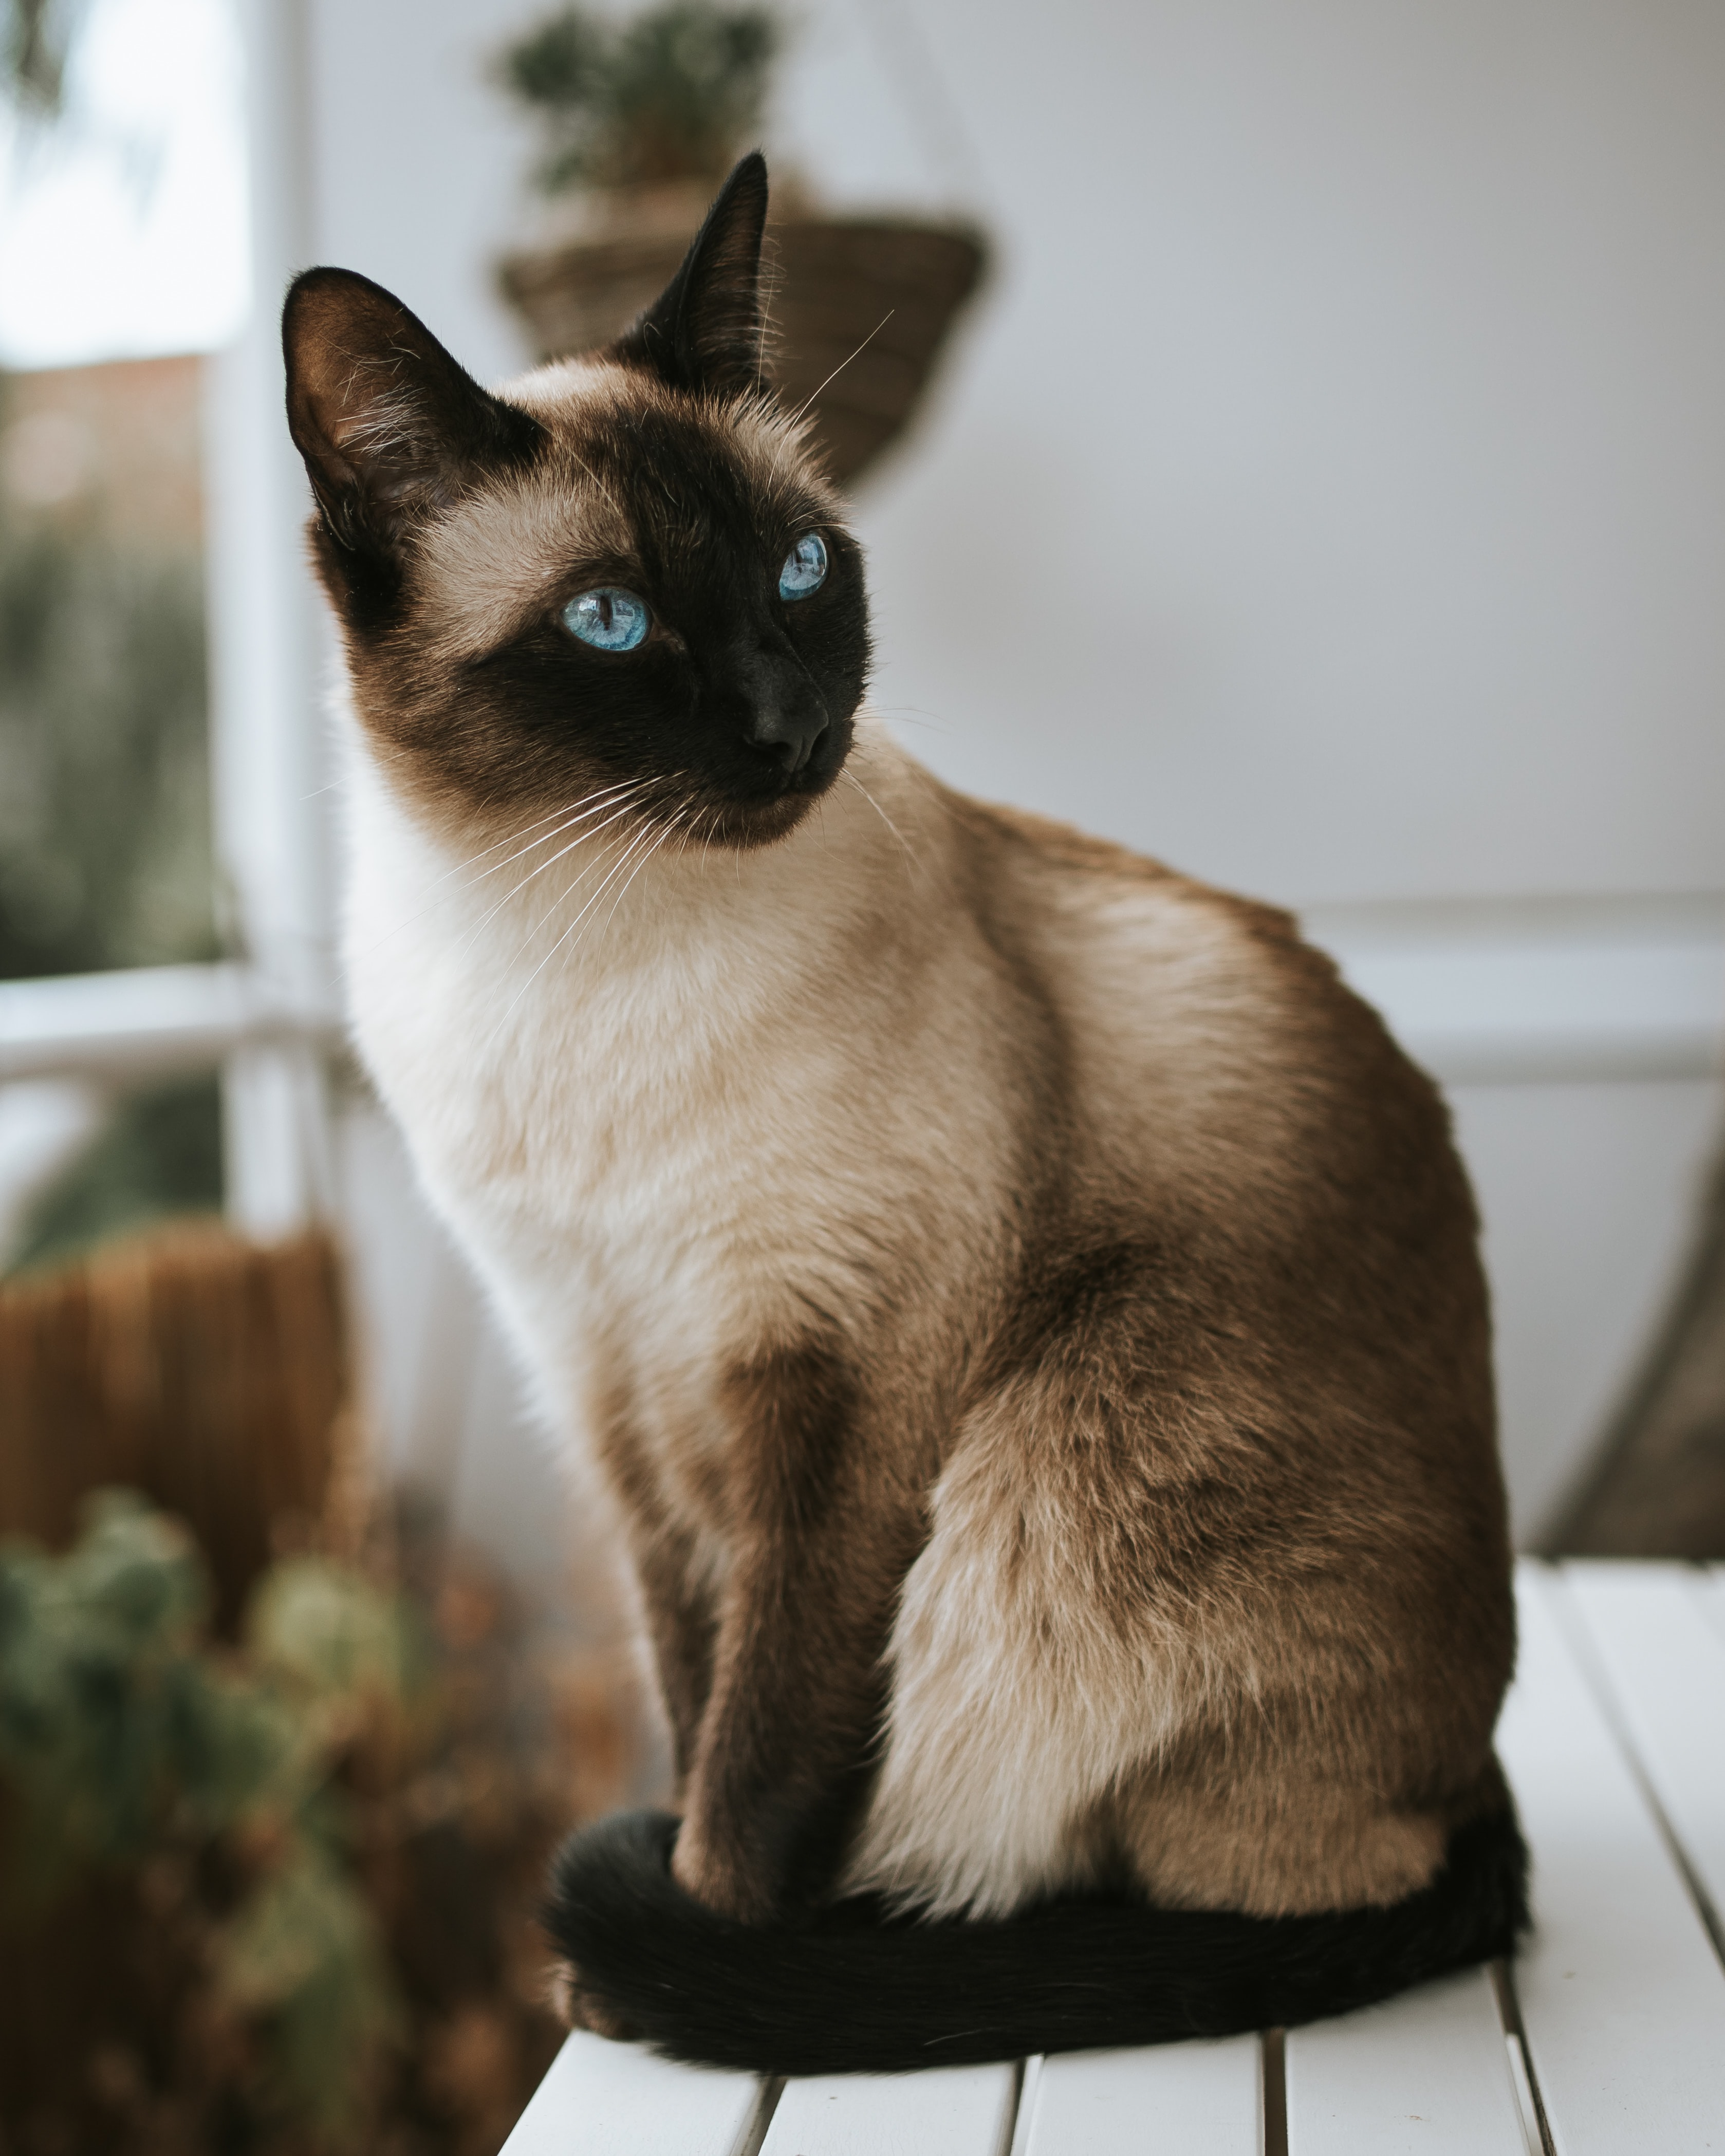
\includegraphics{imagenes/gato_siames.jpg}

}

\subcaption{\label{fig-gato2}Gato 2}

\end{minipage}%

\caption{\label{fig-elephants}Los famosos gatos siames.}

\end{figure}%

Aliquam erat volutpat. Nullam vel augue fringilla, tempor lacus vitae,
viverra magna. Aenean dictum volutpat metus vehicula imperdiet. Donec
vitae placerat purus. Suspendisse potenti. Suspendisse tincidunt at nibh
sit amet pulvinar. Suspendisse non eros dignissim, lacinia justo in,
vulputate magna. Nullam sed libero convallis, consequat nisl sed,
facilisis odio. Nam tincidunt ut arcu id convallis. Donec eget auctor
sem. Mauris in porttitor sem. Mauris id condimentum massa. Aenean
lacinia, mauris sed bibendum laoreet, velit quam fringilla mauris, eu
hendrerit quam libero nec urna. Pellentesque aliquet erat quis ante
commodo lacinia. In quis elit arcu.

\newpage

\textbf{Esquema de metodología}. Sed ut perspiciatis unde omnis iste
natus error sit voluptatem accusantium doloremque laudantium, totam rem
aperiam, eaque ipsa quae ab illo inventore veritatis et quasi architecto
beatae vitae dicta sunt explicabo. Nemo enim ipsam voluptatem quia
voluptas sit aspernatur aut odit aut fugit, sed quia consequuntur magni
dolores eos qui ratione voluptatem sequi nesciunt. Neque porro quisquam
est, qui dolorem ipsum quia dolor sit amet, consectetur, adipisci velit,
sed quia non numquam eius modi tempora incidunt ut labore et dolore
magnam aliquam quaerat voluptatem. Ut enim ad minima veniam, quis
nostrum exercitationem ullam corporis suscipit laboriosam, nisi ut
aliquid ex ea commodi consequatur? Quis autem vel eum iure reprehenderit
qui in ea voluptate velit esse quam nihil molestiae consequatur, vel
illum qui dolorem eum fugiat quo voluptas nulla pariatu.

\begin{figure}

\centering{

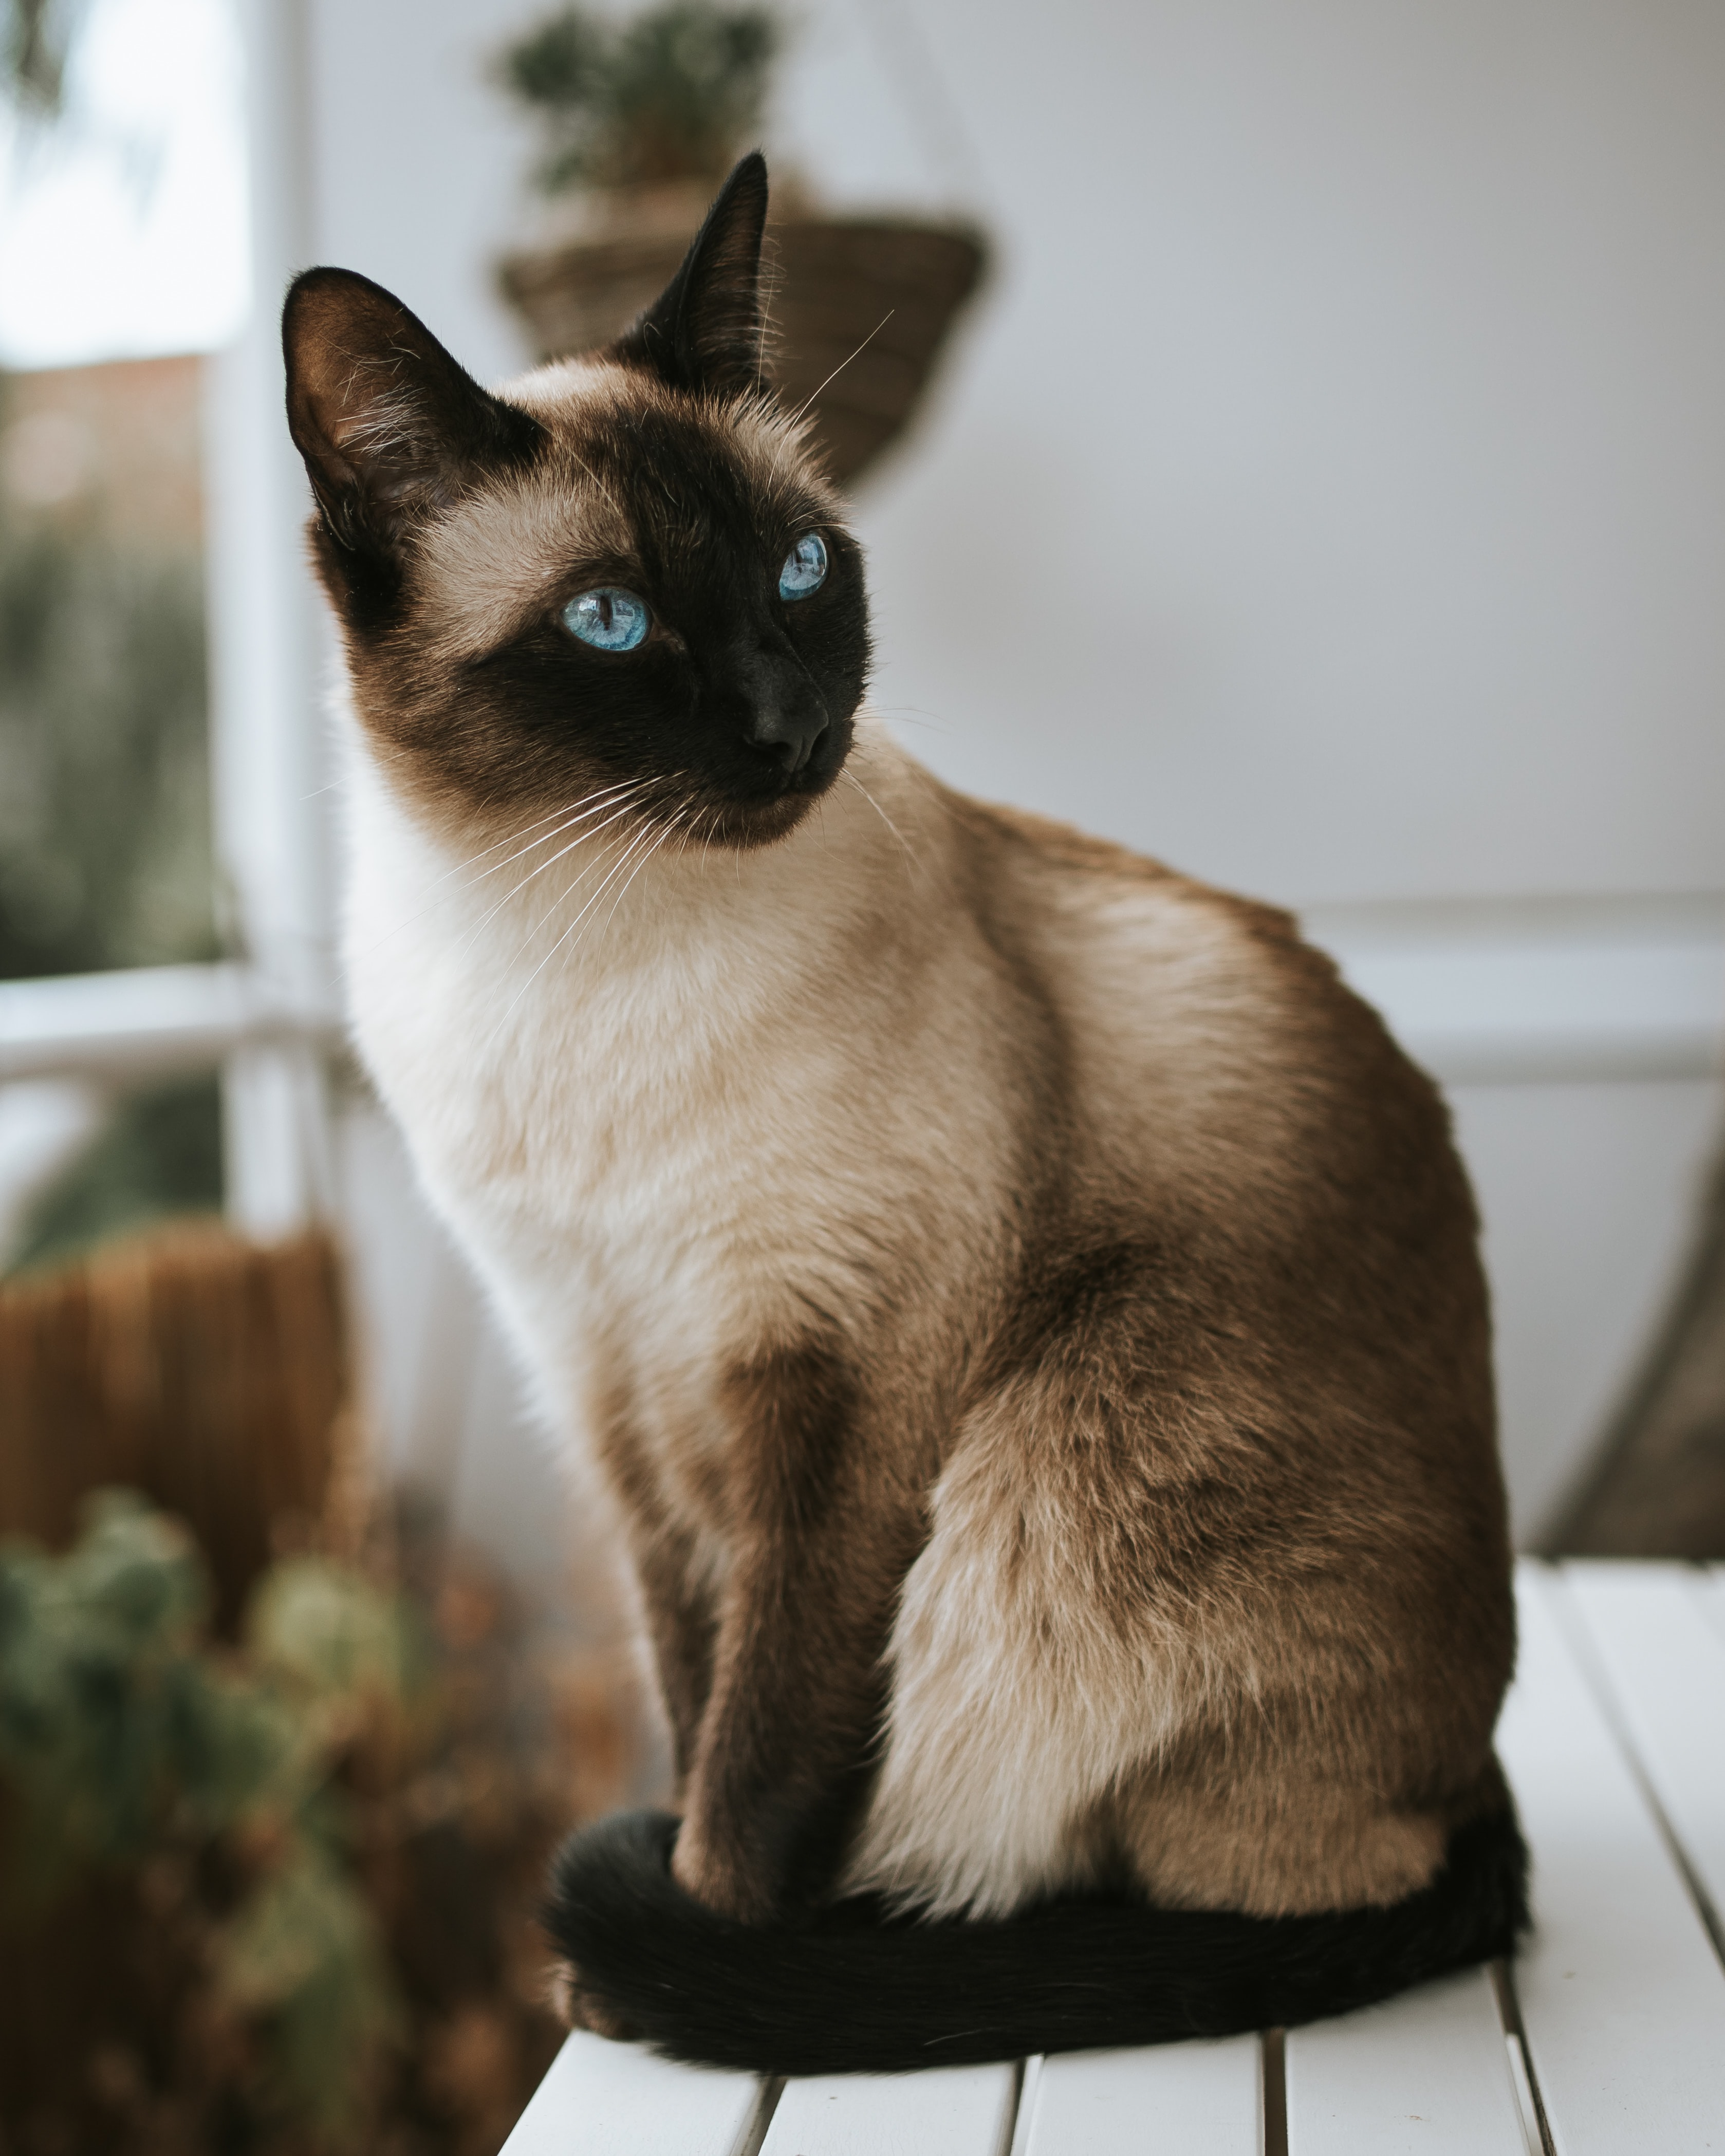
\includegraphics{imagenes/gato_siames.jpg}

}

\caption{\label{fig-metodologia}metodología}

\end{figure}%

\newpage

\bookmarksetup{startatroot}

\chapter{Lorem ipsum dolor sit ame}\label{lorem-ipsum-dolor-sit-ame}

Lorem ipsum dolor sit amet, consectetur adipiscing elit. Suspendisse
sapien nibh, accumsan eu congue vitae, tempus et odio. Aenean porttitor
porta quam, sit amet malesuada ipsum tincidunt quis. Duis id nulla ac
urna suscipit interdum nec vitae sapien. Cras id malesuada augue. Nullam
fermentum, massa at gravida condimentum, erat lacus placerat nisl, quis
placerat metus erat ac nisi. Pellentesque id purus urna. Suspendisse ac
facilisis lacus. Maecenas sit amet quam volutpat tellus dignissim
rutrum. Donec id sodales mauris.

\bookmarksetup{startatroot}

\chapter{Metodología}\label{sec-metodologia}

\bookmarksetup{startatroot}

\chapter{Resultados}\label{sec-Resultados}

Here is an inline note.\footnote{Inlines notes are easier to write,
  since you don't have to pick an identifier and move down to type the
  note.}

Outset content\ldots{}

\begin{tcolorbox}[enhanced jigsaw, toprule=.15mm, opacitybacktitle=0.6, title=\textcolor{quarto-callout-note-color}{\faInfo}\hspace{0.5em}{Nota}, colbacktitle=quarto-callout-note-color!10!white, opacityback=0, breakable, arc=.35mm, toptitle=1mm, leftrule=.75mm, bottomrule=.15mm, titlerule=0mm, coltitle=black, colframe=quarto-callout-note-color-frame, left=2mm, bottomtitle=1mm, colback=white, rightrule=.15mm]

Note that there are five types of callouts, including: \texttt{note},
\texttt{warning}, \texttt{important}, \texttt{tip}, and
\texttt{caution}.

\end{tcolorbox}

\begin{tcolorbox}[enhanced jigsaw, toprule=.15mm, opacitybacktitle=0.6, title=\textcolor{quarto-callout-tip-color}{\faLightbulb}\hspace{0.5em}{Tip With Caption}, colbacktitle=quarto-callout-tip-color!10!white, opacityback=0, breakable, arc=.35mm, toptitle=1mm, leftrule=.75mm, bottomrule=.15mm, titlerule=0mm, coltitle=black, colframe=quarto-callout-tip-color-frame, left=2mm, bottomtitle=1mm, colback=white, rightrule=.15mm]

This is an example of a callout with a caption.

\end{tcolorbox}

Here is some {big text} and some small text.

\bookmarksetup{startatroot}

\chapter{Referencias}\label{referencias}

\phantomsection\label{refs}
\begin{CSLReferences}{1}{0}
\bibitem[\citeproctext]{ref-knuth84}
Knuth, Donald E. 1984. {«Literate Programming»}. \emph{Comput. J.} 27
(2): 97-111. \url{https://doi.org/10.1093/comjnl/27.2.97}.

\end{CSLReferences}



\end{document}
